\chapter{Event Reconstruction}

The energy deposits from the ionized particles traveling through the tracker can also be used to identify the particle species. The track hits reconstructed from the silicon strips can be used to measure the energy deposit $dE/dx$ independently, where $x$ is the thickness of the strip. The particle mass $m$ and the momentum $p$ is related to the energy loss by the formula

\begin{equation}
	\frac{dE}{dx}= K\frac{m^2}{p^2}+C,
\end{equation}
assuming the momenta below the minimum-ionizing region, where $K,C$ are parameters can be extracted from proton line as shown in Fig.~\ref{fig:dedx}.

\begin{figure}[ht]
  \begin{center}
    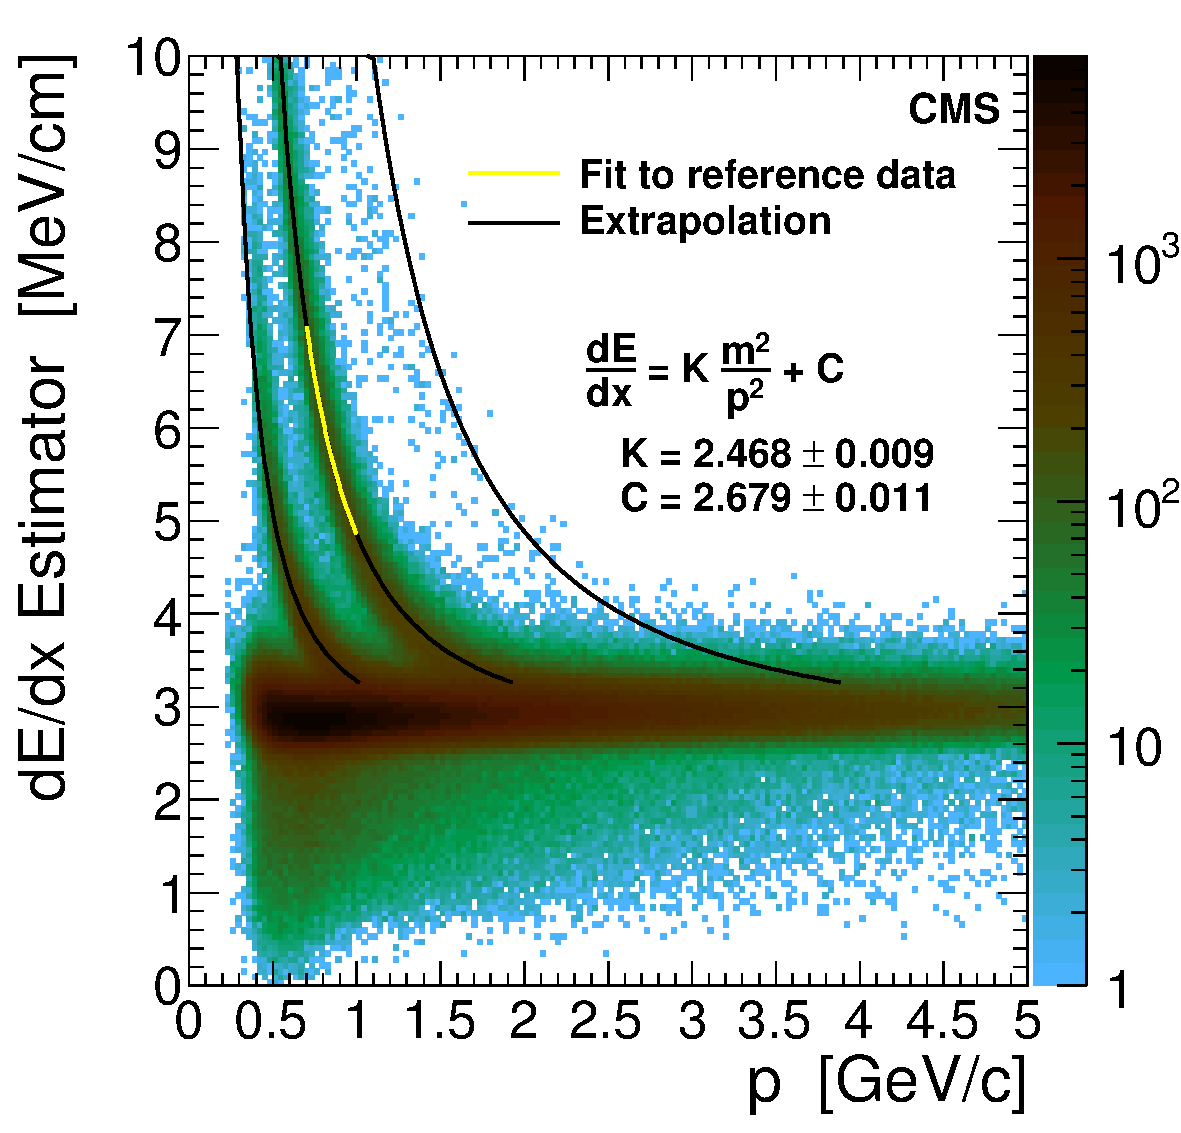
\includegraphics[width=0.6\textwidth]{figures/reconstruction/dedx.pdf}
  \end{center}
  \caption{The Energy loss vs the momentum of tracks. The light yellow curve shows the fitting in the reference range for proton cluster. The rest dark solid lines indicate the extrapolation for kanos, protons, and deuterons. Figure from~\cite{Khachatryan:2010pw}.}
  \label{fig:dedx}
\end{figure}
